\chapter{k-Nearest Neighbour Learning}
\begin{center}
	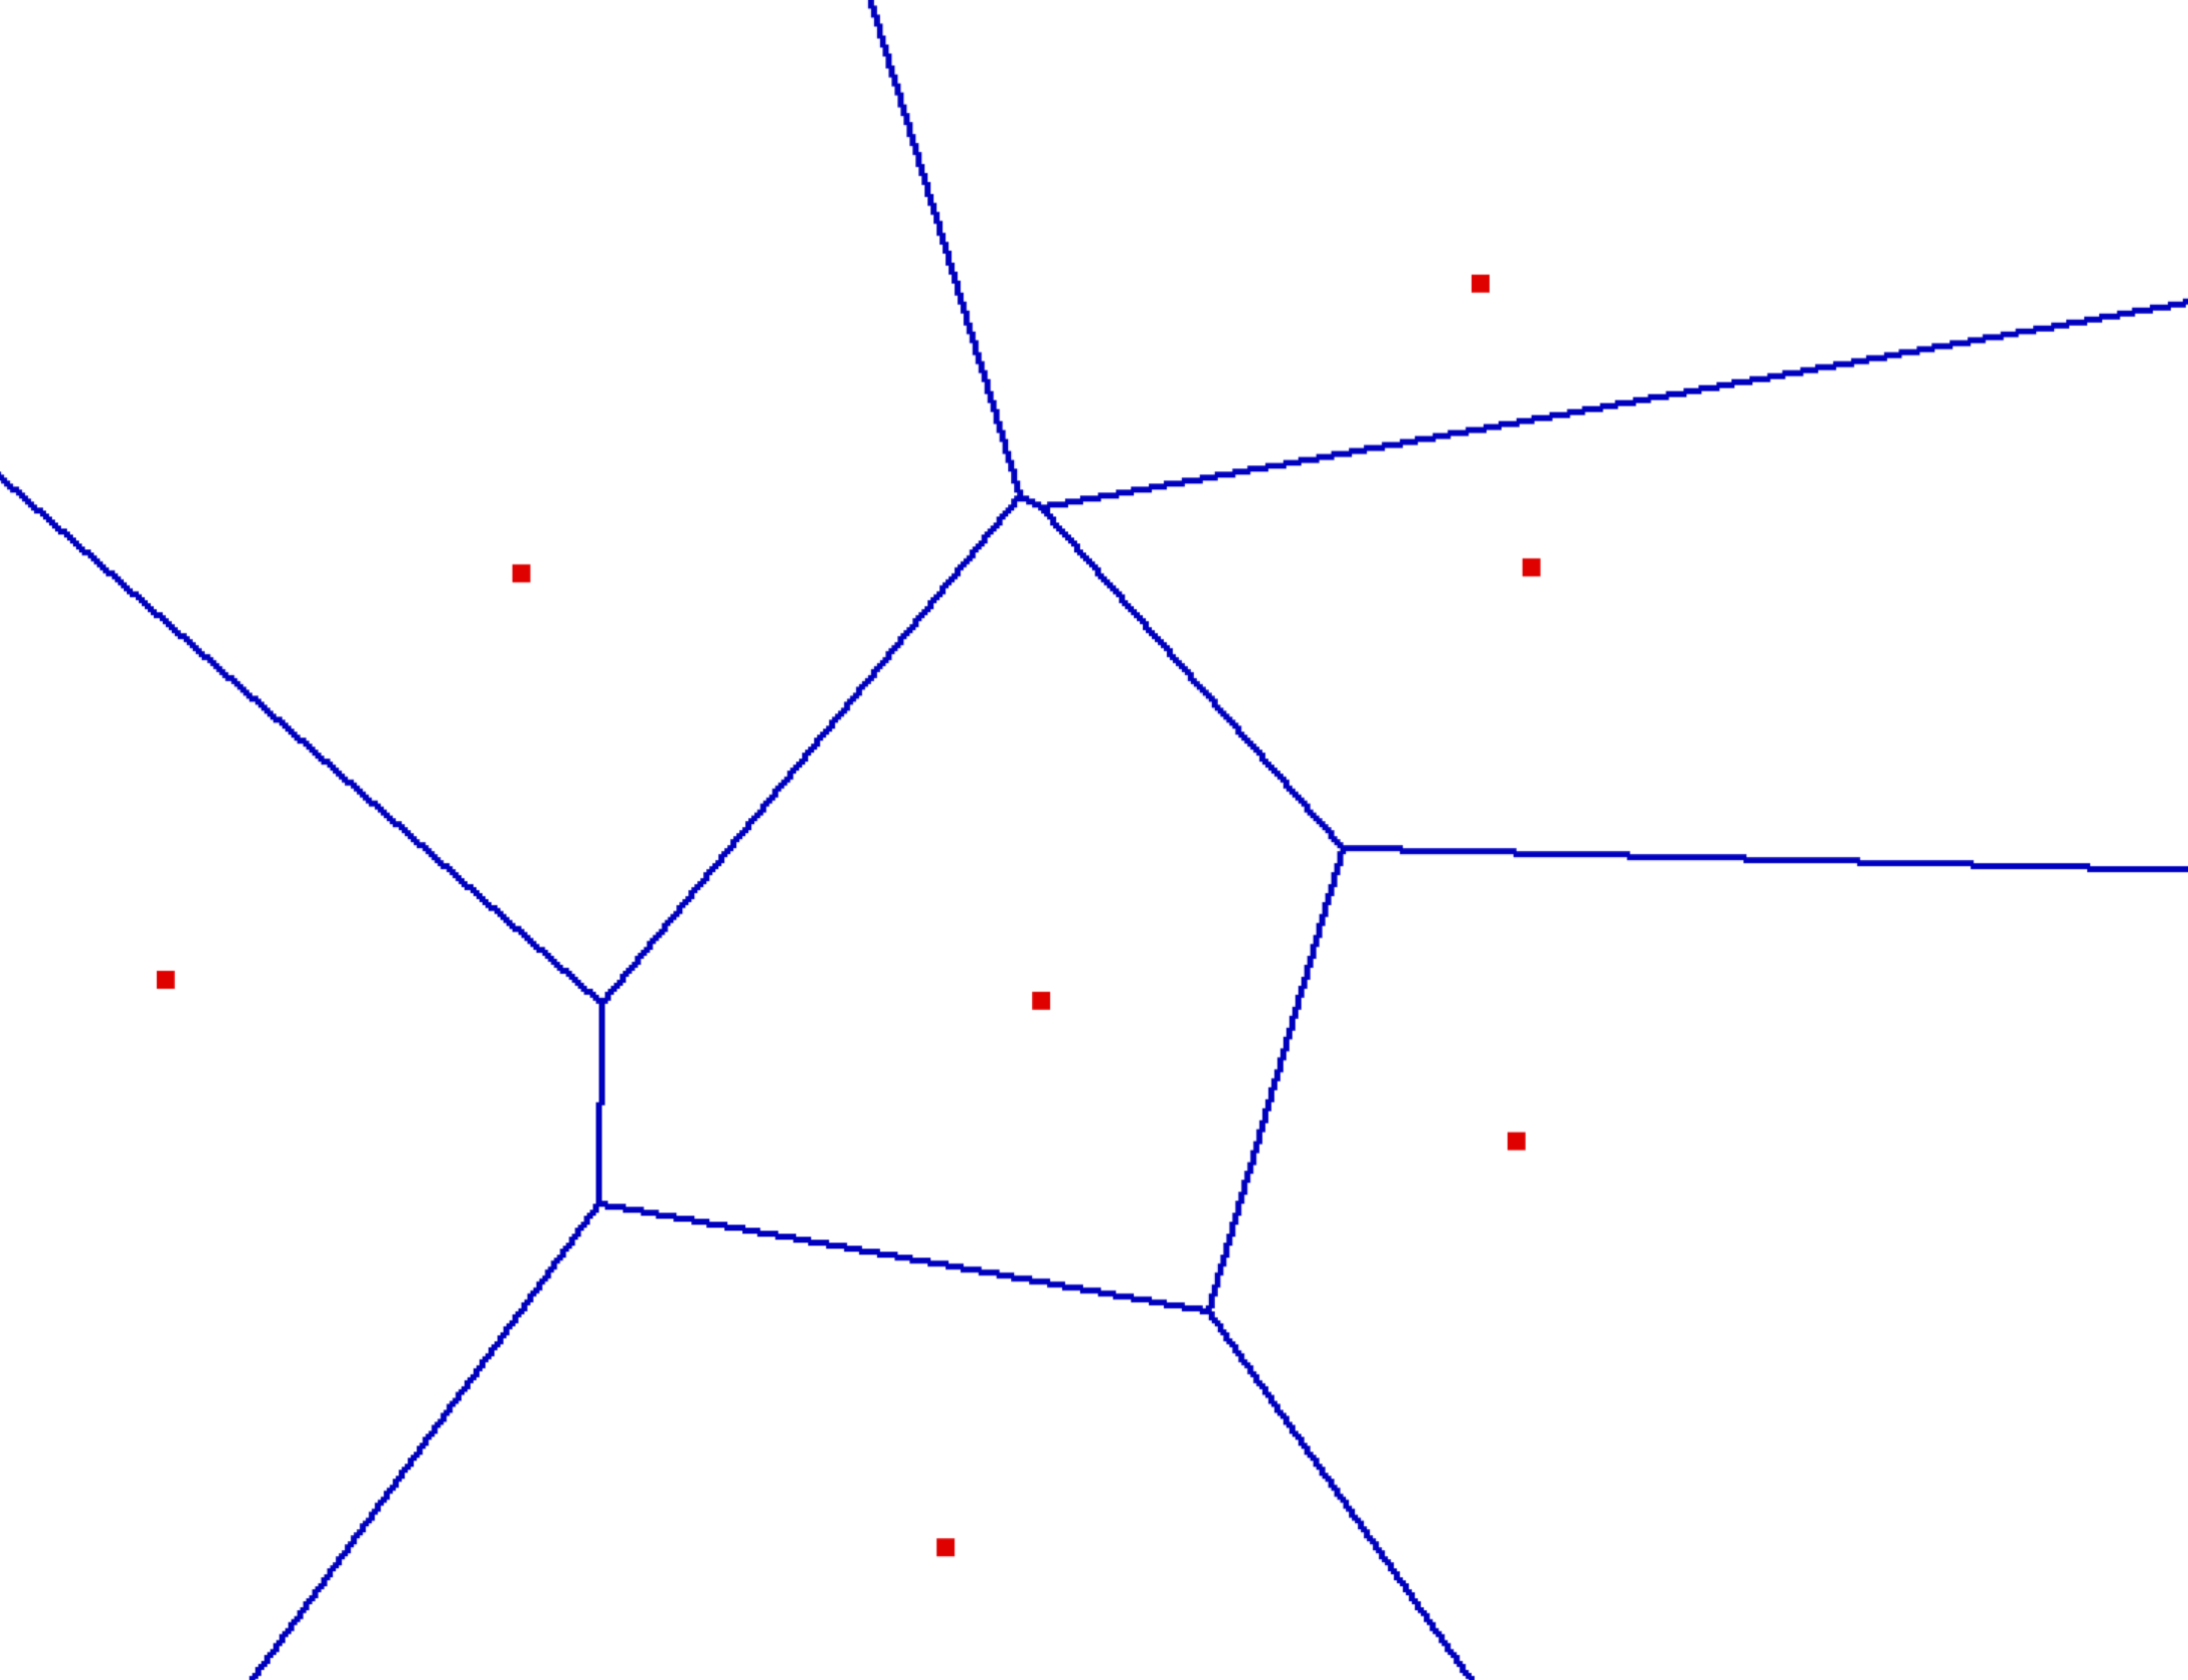
\includegraphics[scale=0.3]{kNearest}
\end{center}
\begin{definition}[Metrics]
Given a set $\mathcal{X}$, a function $d:\mathcal{X}\times\mathcal{X}\rightarrow\mathbb{R}_0^+$ is a \textit{metric} for $\mathcal{X}$ if for any $x, y, z\in\mathcal{X}$ the following properties are satisfied:
\begin{enumerate}
	\item \textbf{Reflixivity}: $d(x,y)=0 \iff x=y$;
	\item \textbf{Symmetry}: $d(x,y)=d(y,x)$;
	\item \textbf{Triangle inequality}: $d(x,y)+d(y,z)\geq d(x,z)$
\end{enumerate}
\end{definition}
A frequently used, and well-known, function $d$ is the Euclidean distance defined in $\mathbb{R}^n$:
\begin{center}
	$\displaystyle d(x, y)=\sqrt{\Sum_{i=1}^n(x_i-y_i)^2}$
\end{center}
%
%
%
\section{The algorithm}
%
%
\subsection{Classification problem}
\begin{lstlisting}
for all test examples x do
	for all training examples %*$(x_i, y_i)$*) do
		compute distance %*$d(x, x_i)$*)
	end for
	select the k-nearest neighbours of x
	return class of x as majority class among neighbours:
		%*$\text{argmax}_y\Sum_{i=1}^k\delta(y, y_i)$*)
end for
\end{lstlisting}
Where 
\[
\delta(x,y)=
\begin{cases}
	1\quad \text{if}~x=y\\
	0\quad \text{otherwise}
\end{cases}
\]
%
%
\subsection{Regression problem}
\begin{lstlisting}
for all test examples x do
	for all training examples %*$(x_i, y_i)$*) do
		compute distance %*$d(x, x_i)$*)
	end for
	select the k-nearest neighbours of x
	return the average output value among neighbours:
		%*$\displaystyle \frac{1}{k}\Sum_{i=1}^ky_i$*)
end for
\end{lstlisting}
%
%
%
\section{Characteristics}
\begin{itemize}
	\item \textbf{Instance-based learning}: the model used for prediction is calibrated for the test example to be processed;
	\item \textbf{Lazy learning}: computation is mostly deferred to the classification phase;
	\item \textbf{Local learner}: assumes prediction should be mainly influenced by nearby instances;
	\item \textbf{Uniform feature weighting}: all features are uniformly weighted in computing distances.
\end{itemize}























